\chapter{Exportando dados}

Com o InVesalius, é possível exportar dados para outros softwares, em formatos de arquivo
como OBJ, STL, entre outros.

O menu que contém as opções para exportação localiza-se no painel esquerdo do InVesalius,
dentro do item \textbf{4. Exporte os dados}. Caso o menu não esteja visível, dê um clique
duplo com o botão \textbf{esquerdo} do mouse sobre o item para expandi-lo. A figura
\ref{fig:data_export} mostra esse menu.

\begin{figure}[!htb]
\centering
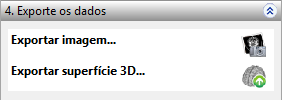
\includegraphics[scale=0.8]{../user_guide_figures/invesalius_screen/painel_data_export_pt.png}
\caption{Menu para exportação de dados}
\label{fig:data_export}
\end{figure}

\section{Superfície}

Para exportar uma superfície, é necessário selecioná-la no menu de dados, conforme mostra a
figura \ref{fig:data_export_selection}.

\newpage

\begin{figure}[!htb]
\centering
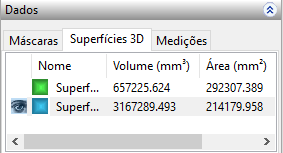
\includegraphics[scale=0.7]{../user_guide_figures/invesalius_screen/painel_data_export_selection_pt.png}
\caption{Seleção de superfície a exportar}
\label{fig:data_export_selection}
\end{figure}

Em seguida, clique sobre o ícone que a figura \ref{fig:surface_export_original} ilustra.

\begin{figure}[!htb]
\centering

\includegraphics[scale=0.2]{../user_guide_figures/icons/surface_export_original.png}
\caption{Atalho para exportar superfície}
\label{fig:surface_export_original}
\end{figure}

Na janela exibida (figura \ref{fig:export_data_window}), insira o nome do arquivo e
selecione o formato desejado para a exportação. Em seguida, clique em \textbf{Salvar}.


\begin{figure}[!htb]
\centering
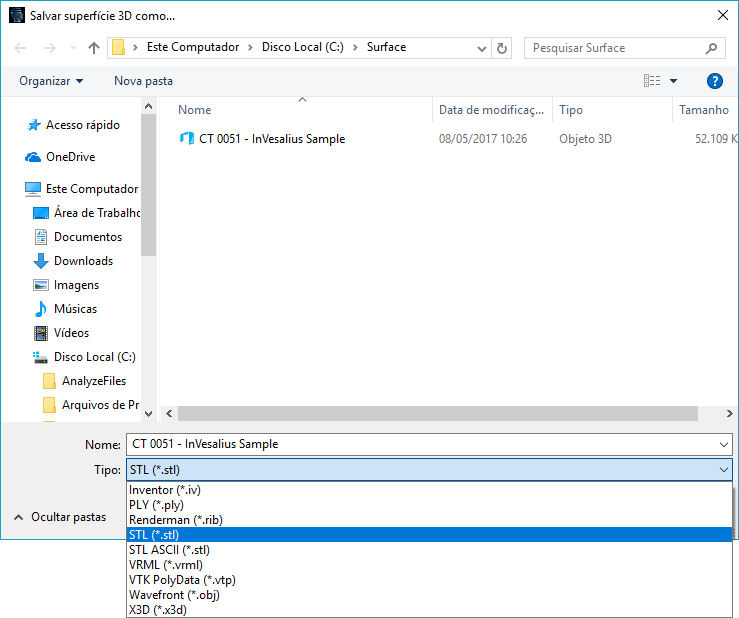
\includegraphics[scale=0.4]{../user_guide_figures/invesalius_screen/export_surface.png}
\caption{Janela para exportar superfície}
\label{fig:export_data_window}
\end{figure}

Os tipos de arquivo que podem ser exportados estão listados na tabela
\ref{tab:files_export_list}:

\begin{table}[h]
\centering
\caption{Formatos de arquivo que o InVesalius exporta}
\begin{tabular}{lcc}\\
\hline % este comando coloca uma linha na tabela
Formato & Extensão\\
\hline
\hline
Inventor & .iv\\
Polygon File Format & .ply\\
Renderman & .rib\\
Stereolithography (formato binário)& .stl\\
Stereolithography (formato ASCII) & .stl\\
VRML & .vrml\\
VTK PolyData & .vtp\\
Wavefront & .obj\\
\hline
\end{tabular}
\label{tab:files_export_list}
\end{table} 


\section{Imagem}

É possível exportar imagens de qualquer das orientações de exibição (axial, coronal,
sagital e 3D). Para isso, clique com o botão \textbf{esquerdo} do mouse sobre o atalho
exibido na figura \ref{fig:menu_save_image_window} e selecione a sub-janela correspondente
à imagem que deseja exportar.

\begin{figure}[!htb]
\centering
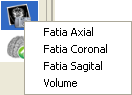
\includegraphics[scale=0.5]{../user_guide_figures/invesalius_screen/menu_save_image_window_pt.png}
\caption{Menu para exportar imagem}
\label{fig:menu_save_image_window}
\end{figure}

Na janela exibida (figura \ref{fig:save_image_window}), selecione o formato do arquivo e
clique no botão \textbf{Salvar}.

\begin{figure}[!htb]
\centering
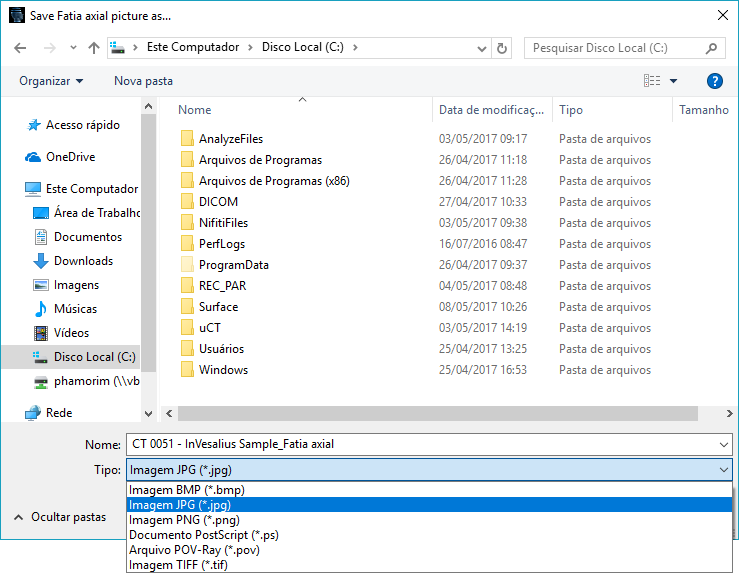
\includegraphics[scale=0.4]{../user_guide_figures/invesalius_screen/export_bmp_pt.png}
\caption{Janela para exportar imagem}
\label{fig:save_image_window}
\end{figure}
